\documentclass[12pt]{article}
\ProvidesPackage{preamble}

%% General formatting
\usepackage{enumerate}
\usepackage{amsmath}
\usepackage{breqn}
\usepackage{bbm}
\usepackage[margin=1in]{geometry}
\usepackage[hidelinks]{hyperref}
\usepackage{subfiles}
\usepackage{setspace}
\usepackage{graphicx}
\usepackage[labelfont=bf]{caption}
\usepackage{hhline}
\usepackage{threeparttable}
\usepackage{tabularx}
\usepackage{parskip}

% %% Beamer Stuff
% \usepackage{appendixnumberbeamer}å

%% Bibliography packages
\usepackage{natbib}
\bibliographystyle{abbrvnat}
\setlength\parindent{0pt}
\onehalfspacing

\title{The 1885 Chinese Head Tax and Immigration to Canada}
\author{Amy Kim}

\begin{document}
\maketitle

\section{Introduction}
While work on the effect of historical immigration policies in the US has begun to develop in recent years, there is still a large dearth of research on similar policies in Canada. In this paper, I focus on a discriminatory `Head Tax' on Chinese immigrants to Canada during the late 19th and early 20th centuries. This policy used a lump-sum monetary disincentive that was unique to Chinese immigrants to explicitly discourage Chinese immigration, while not outright banning immigration (as the US did during the same time period). The head tax, initially a \$50 entry fee, evolved to a \$500 entry fee, which was prohibitively expensive for many immigrants at the time.

While some researchers have studied historical anti-Chinese immigration policy \citep{Chen2015, ChenXie2020, Postel2023}, with meaningful results, no one to my knowledge has looked specifically at the Chinese Head Tax in Canada. Analyzing the effects of this policy on Chinese immigration inflow to Canada, and the subsequent effects of this policy on the characterstics of Chinese immigrants after arrival (whether through selection into immigration or through the wealth effects of the tax) will not only shed light on the past, but will also inform policymakers today about the consequences of immigration costs (whether explicit or implicit) on immigration inflow and immigrant outcomes.

In this paper, I find evidence that the Chinese Head Tax \textbf{did} have significant effects on Chinese immigration inflows to Canada. I also analyze outcomes for Chinese immigrants to Canada, and find evidence that the head tax had a strong negative impact on home ownership compared to other immigrant groups, even after controlling for China-side immigrant supply effects by using data on US immigrants. 
I also find evidence that the head tax increased the likelihood of Chinese immigrants being literate and decreased their likelihood of working as a laborer, suggestive of a positive effect on selection into migration (i.e. more skilled immigrants became relatively more likely to immigrate as the head tax increased). I also look at earnings, and find that effects are positive when compared to all immigrants (suggestive of a selection effect) but when compared to only Japanese immigrants, effects are negative.

Section 2 of this paper provides more historical context on the Chinese Head Tax in Canada as well as anti-Chinese immigration policy in the US at the time, section 3 describes the data sources I use for my analysis, and section 4 presents some preliminary results.


\section{Background and Historical Context}
Although the history of Chinese immigration to North America reaches back to the 1700s, it was not until the Gold Rush of the 1850s that large numbers of Chinese immigrants began to settle along the West Coast. 
While initially concentrated in California, later discoveries of gold in British Columbia expanded Chinese immigration to Canada, and by 1860 there were an estimated 7,000 Chinese inhabitants of British Columbia \citep{chan2019}.
Following the Gold Rush, Chinese immigrants largely took on low-wage jobs in the manufacturing and service industries, and in 1880-1885 contributed heavily to the construction of the Canadian Pacific Railway.
As the completion of the railway approached, however, sinophobic sentiment began to foment, and in 1884 a commission was formed to investigate the possibility of restricting Chinese immigration to Canada \citep{chan2016}.

\subsection{Chinese Head Tax in Canada}
With the passage of the Chinese Immigration Act of 1885 came a \$50 `Head Tax' -- a per-person entry fee for all immigrants from China. While the commission appointed to investigate Chinese immigration had originally suggested a \$10 head tax, intended to pay for a health inspector at entry ports,
it was clear that the \$50 fee was implemented with the goal of dissuading Chinese immigrants from settling in Canada. 50 CAD in 1885 would be worth approximately 1,500 USD in 2023, and at the time was nearly a fifth of the average Chinese immigrant's yearly salary.
As Chinese immigration to Canada continued to grow despite the tax, the government raised the tax to \$100 in 1900 (approximately 3,500 USD in 2023) and to \$500 in 1903 (approximately 17,000 USD in 2023). 

The Chinese Immigration Act also limited the capacity of incoming ships carrying Chinese passengers (with no changes to capacity for incoming ships carrying European passengers) and while exceptions to the tax were made for diplomats, merchants, students, and others, the vast majority of Chinese immigrants were forced to pay the tax. 
Failure to do so would result in being sent back to China, and as a result many immigrants had to either borrow money or enter indentured servitude contracts to cover the cost of the tax. 
The tax remained in place until 1923, when the Chinese Immigration Act of 1923 banned Chinese immigration to Canada altogether until its repeal in 1947.

\subsection{Chinese Immigration to the US}
Chinese immigration to the US evolved in a similar way as Canada throughout the 19th century, beginning with the Gold Rush, growing through the construction of the Transcontinental Railroad, and culminating in the Chinese Exclusion Act of 1882.
The legislation in the US, however, took a more severe approach than the Canadian counterpart, completely banning the immigration of Chinese laborers, a ban which remained in place until 1943. 
While there are some accounts of immigrants from China landing in Canada and crossing the border by land into the US, estimates suggest that the Exclusion Act did heavily limit the growth of the Chinese population in the US, particularly for low-wage workers.

\section{Data}
\subsection{Description of Data Sources}

\subsubsection{Chinese Register}
The first and primary source of data that I use is the Register of Chinese Immigrants to Canada\footnote{Data is obtained from \citet{chineseregister}.}, 
which is a record maintained from 1885 to 1949 of all Chinese immigrants to Canada.
The Register includes the full name, amount of tax paid, age and sex, occupation, place of origin within China, port and date of arrival, among other variables. 
In addition to serving as a full count of immigrants of Chinese origin who \textit{entered} Canada during the years affected by the head tax,
the Register also records any Chinese immigrants who had already entered Canada prior to the implementation of the Chinese Immigration Act in 1885 (and therefore were not subject to the tax),
but chose to pay the tax and register with immigration authorities so that they could exit and re-enter the country without paying additional fees.
Although this dataset allows me to precisely observing the timing of entry into Canada, it does not record the outflow of Chinese immigrants, and so it does not accurately capture the stock of Chinese immigrants in Canada in any given year.
Additionally, this dataset is likely to miscount Chinese immigrants who entered illegally or under a false name.

\subsubsection{Canadian Census}
Microdata from historical Canadian censuses are currently available through 1921.\footnote{Data are compiled from \citet{census1901}, \citet{census1911}, \citet{census1921}, for the 1901, 1911, and 1921 censuses respectively. Note that while data from the 1852, 1871, 1881, and 1891 censuses are also available, none contain the variable Year of Immigration, making it difficult to measure the impact of the head tax (which went into effect and changed dollar amounts between census years). As a result, these earlier censues are excluded from this analysis.} 
Unfortunately, only 4-5\% of these censuses have been digitized (with random sampling). While this data source provides a rich set of variables, the low sampling rate results in a very small sample size for Chinese immigrants, who were already a relatively small percentage of the Canadian population at the time. 
Since the census only took place every ten years, this data source provides a cross-sectional view of the country at different points in time, acting as a complement to the data on inflows from the Chinese Register.
Section 3.2 compares these two datasets in further detail.

\subsubsection{US Census}
Finally, I also use US census data in my analysis. I use full-count census data from the 1900-1920 US censuses,\footnote{All data is obtained from \citet{ipums}.} which, much like the Canadian census data, serves as a cross-sectional view of the Chinese immigrant population in the US at different points in time.

\subsection{Comparing Data Sources}

\begin{table}[!h]
    \centering 
    \renewcommand{\arraystretch}{1.5}
    \resizebox{\textwidth}{!}{
    \begin{threeparttable}
        \caption{Summary statistics for pooled Canadian census data (1901-1921), pooled US census data (1900-1920), and the Chinese Register, grouped separately by the entire population, the entire immigrant population, and the Chinese immigrant population.}
        \label{tab:summstats}
        % latex table generated in R 4.0.3 by xtable 1.8-4 package
% Mon Oct 10 23:48:19 2022
\begin{tabular}{lccc}
  \hline
 & CA Census (1901-1921) & Chinese Registry (1885-1924) & US Census (1900-1920) \\ 
  \hline
\% Male & 0.98 & 0.98 & 0.95 \\ 
   & (0.16) & (0.15) & (0.21) \\ 
  \% Married & 0.55 & - & 0.44 \\ 
    & (0.5) & - & (0.5) \\ 
  Avg. Age at Imm & 23.20 & 25.95 & 20.92 \\ 
     & (8.99) & (21.86) & (9.78) \\ 
  \% Can Read & 0.68 & - & 0.77 \\ 
        & (0.47) & - & (0.42) \\ 
  \% Labourers & 0.20 & 0.62 & 0.32 \\ 
           & (0.4) & (0.48) & (0.47) \\ 
   \hline
Obs &   4230 &  90946 & 186523 \\ 
   \hline
\end{tabular}

        \begin{tablenotes}
            \item *Calculated as a percentage of adults. 
            
            \item \textbf{Notes:} Column (1) pools Canadian census data (as described in section 3.1.2) from 1901, 1911, 1921, calculating means and standard errors of each variable for the whole population, weighted based on the coverage of that year's census (5\% for 1901-1911, and 4\% for 1921). The small number of observations for Canada relative to the US is due to this sampling structure.
            Column (3) repeats this exercise for individuals born outside of Canada, and Column (5) repeats this exercise for individuals born in China. Column (2) pools American census data (as described in section 3.1.3) from 1900, 1910, 1920 to calculate means and standard errors of each variable for the full population -- note that since these censuses all have 100\% coverage, there is no population weighting.
            Column (4) repeats this exercise for individuals born outside of the US, and Column (6) repeats this exercise for individuals born in China. Finally, column (7) uses the entire Chinese Register (as described in section 3.1.1) to calculate means and standard errors of each variable for the population of Chinese immigrants to Canada recorded in the Chinese Register. Matched immigrants in columns (8) are non-Chinese immigrants from Canadian census years 1901-1921, matched to Chinese immigrants from the 1881 Canadian census. Matched immigrants in columns (9) are non-Chinese immigrants from a 1\% sample of the US census in years 1900-1920, matched to Chinese immigrants from a 10\% sample of the 1880 US census (sampling done for computational reasons).
        \end{tablenotes}
    \end{threeparttable}
    }
\end{table}

Table \ref{tab:summstats} compares summary statistics across the different data sources, for the entire population, the entire immigrant population, and the Chinese immigrant population. Columns (1) and (2) compare the entire population of Canada, as summarized in the Canadian censuses from 1901-1921, to the entire population of the US, as summarized in the US censuses from 1900-1920. There are very small differences in characteristics between the two groups, suggesting that the general population of the two countries was very similar over this time period. 

Columns (3) and (4) compare the immigrant populations of the two countries. While also largely similar in terms of the gender distribution (slightly more male than the overall population), marital status (slightly more likely to be married than the overall population), there are several differences. The first and most significant is the difference in year of immigration -- immigrants to Canada immigrated nine years later on average. Additionally, while immigrants in both countries are older than the overall population, this is more pronounced in the US, and immigrants to the US are slightly less likely to be literate in English. 

Columns (5) and (6) compare the Chinese immigrant population of the US and Canada, focusing on those who immigrated after 1885. Observe that many of the differences between these two columns could be explained by the enforcement of the Chinese Exclusion Act in the US starting in 1882: as the inflow of lower-skilled Chinese laborers stops, the fraction of laborers in the Chinese immigrant population drops, the likelihood of literacy increases, the average age increases, and the population is slightly less male. Note, however, that this explanation does not account for the differences in likelihood of being married, and furthermore, the presence of some laborers in the post-1885 US sample suggests imperfect compliance to the Chinese Exclusion Act. 

Finally, column (7) summarizes available data from the Chinese Register. The results show that while the immigrants recorded in the Chinese Register are similarly male and arrive at similar times as the Chinese immigrants recorded in the Canadian census, they are much younger and also possibly more likely to be laborers.\footnote{For census data, I directly impute laborer status as a function of occupational group, which is encoded differently across censuses, and is therefore not directly comparable to the laborer variable in the Chinese Register, where ``Laborer'' was a category of occupation that was directly recorded. Additionally, this variable in the Chinese Register was recorded at the time of entry, and does not reflect the occupation an immigrant may have had after arrival in Canada.}
Note that the key difference between the Canadian census and the Register is that while the Register counts each (legal) entry into the country, the census is cross-sectional and therefore does not count immigrants who both arrive and subsequently leave the country between censuses. Indeed, a simple accounting exercise shows that between 1911 and 1921, the population of Chinese immigrants represented in the census grew by nearly 10,000, while in the same time period, the Chinese Register recorded the arrival of over 29,000 Chinese immigrants, implying a net outflow of 19,000 Chinese immigrants. Repeating this same exercise implies similarly large outflows in other decades in this period. 


\section{The Effects of the Chinese Head Tax}

\begin{figure}
    \centering 
    \caption{Average non-zero tax paid by Chinese immigrants to Canada, by year of arrival in Canada, as reported in the Chinese Register.}
    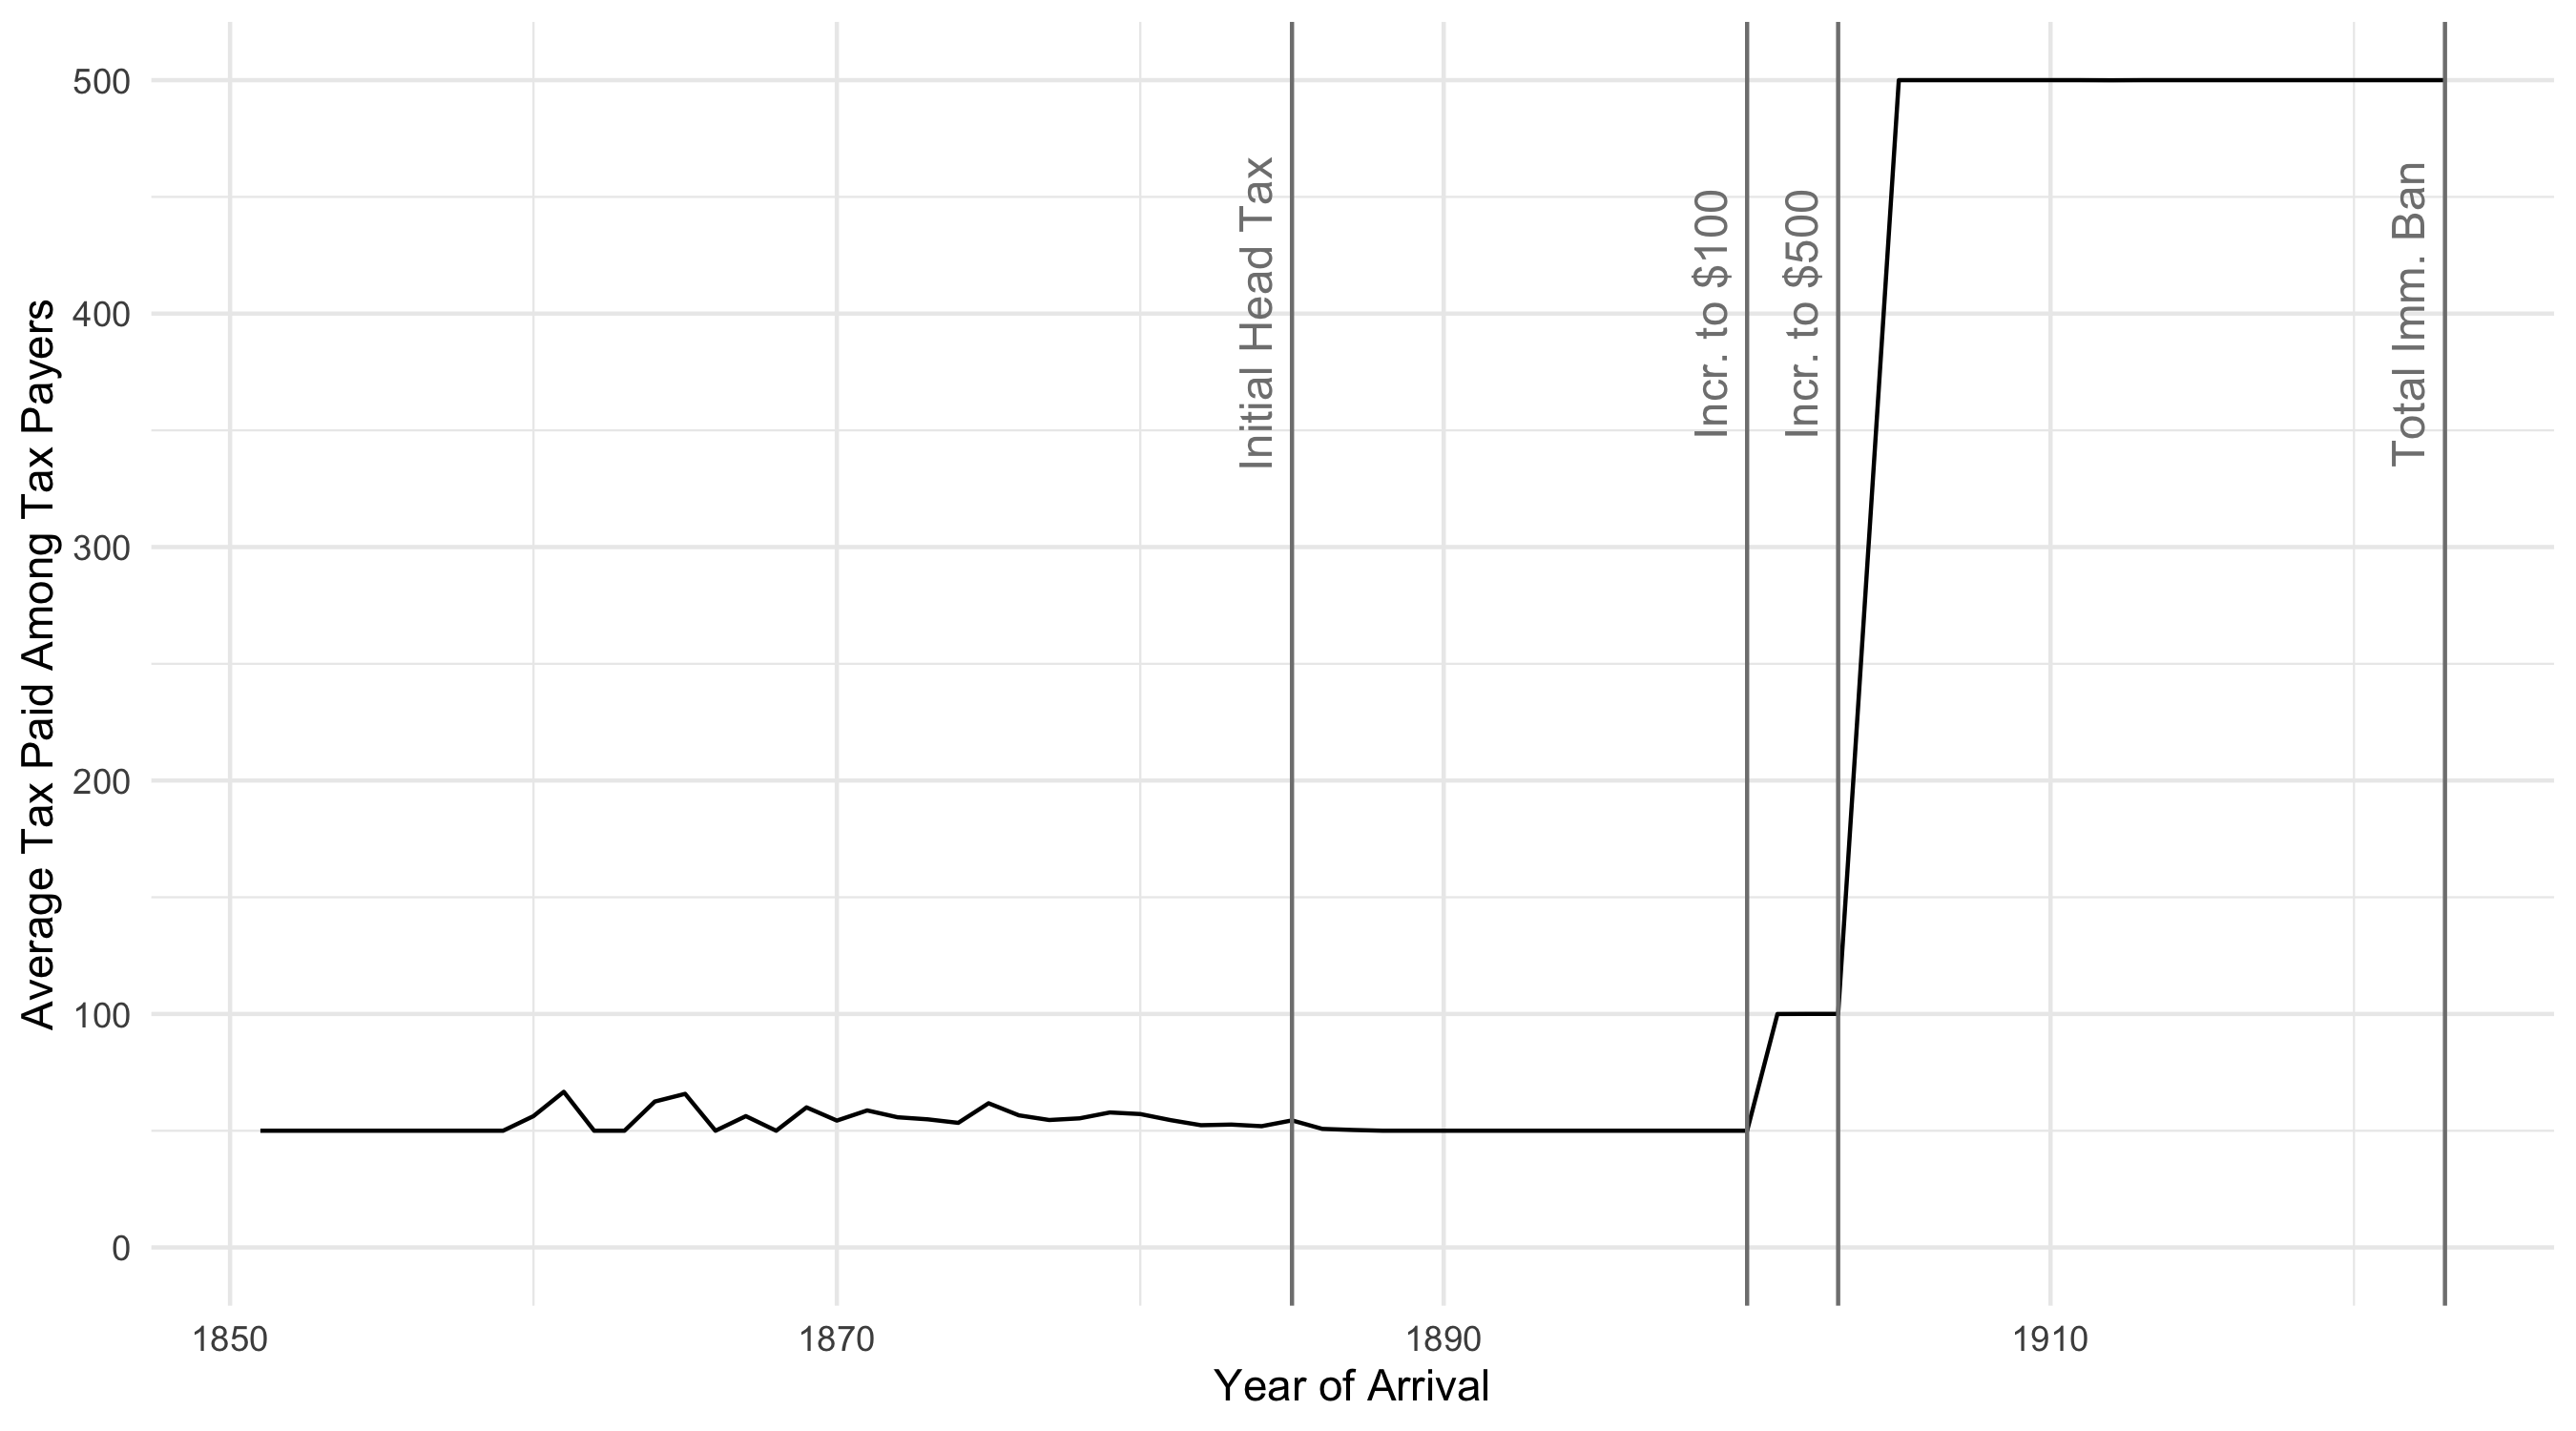
\includegraphics[width=\textwidth]{../../figs/shortpaper_figs/fig1_taxespaid.png}
    \label{fig:taxpaid}
\end{figure}

I begin by documenting the average non-zero tax paid by Chinese immigrants in each year, as recorded in the Chinese Register, in Figure \ref{fig:taxpaid}.\footnote{Note that only 8.7\% of pre-1923 arrivals recorded in the Chinese Register paid \$0 in taxes. Of these non-taxpaying individuals, approximately 89\% were merchants or the family of a merchant, and an additional 4\% were students or working in other professions exempt from the tax.} The figure suggests nearly perfect adherence to the Chinese Head Tax by port officials, with immigrants entering between 1885 and 1900 paying \$50, immigrants entering between 1900 and 1903 paying \$100, and immigrants entering between 1903 and 1923 paying \$500. Small spikes prior to 1885 indicate the existence of some immigrants who arrived prior to 1885 and subsequently registered in or after 1885 who were required to pay more than \$50 (approximately 6\% of all immigrants in the Register data who arrived prior to 1885) -- the reason for this is unclear. 

While the Register does not account for immigrants who entered without registration, there is reason to believe that this was a rare occurence. At the time, the only way for Chinese immigrants to arrive in Canada was by ship, since the US at the time had even stricter restrictions on Chinese immigration.\footnote{There are even some accounts of Chinese immigrants arriving by ship in Canada and attempting to cross the border \textit{into the US }by land, to circumvent the Chinese Exclusion Act in the US.} Since shipping ports were much better surveilled than land borders, it is unlikely that many would have been able to enter without registering. 


\subsection{Effects on Migration}

\begin{figure}
    \centering 
    \caption{Inflow of Chinese immigrants to Canada, as measured by the Chinese Register and the Canadian census.}
    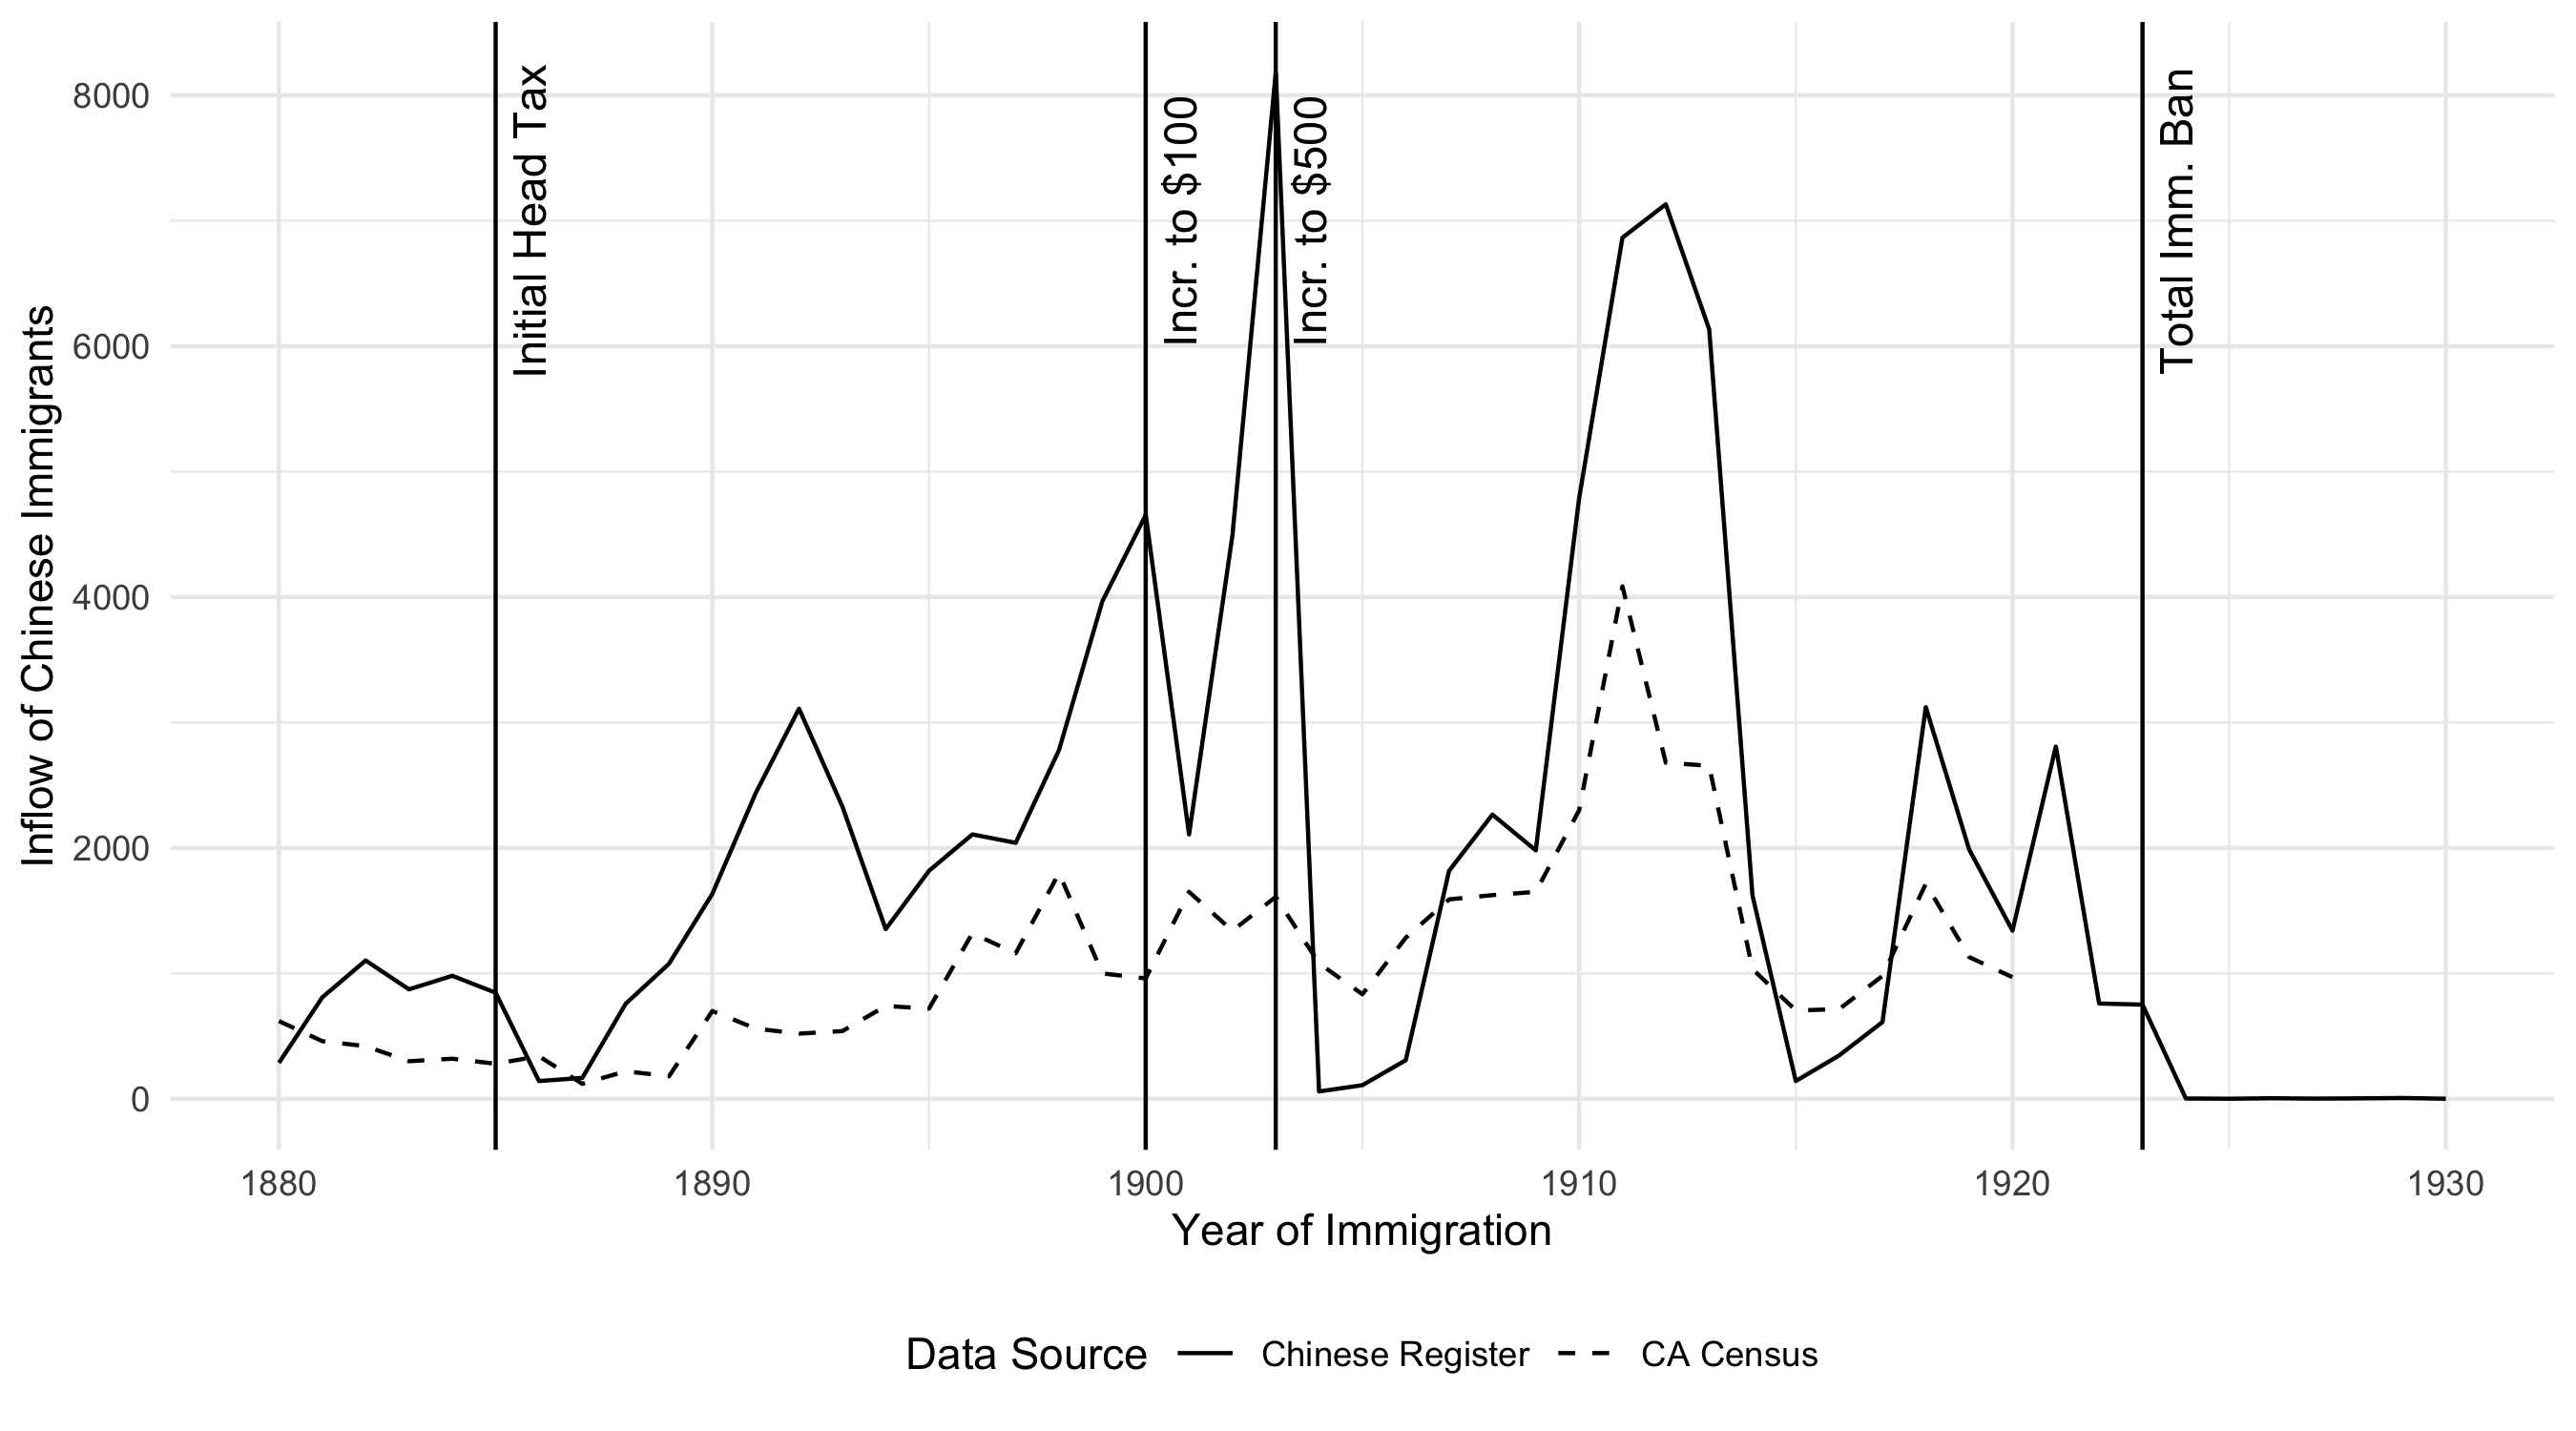
\includegraphics[width=\textwidth]{../../figs/shortpaper_figs/fig2_flow.png}
    \label{fig:inflow}
\end{figure}

Figure \ref{fig:inflow} shows the flow of immigrants into Canada between 1880 and 1930, as documented longitudinally in the Chinese Register, and as documented by repeated cross-section in the Canadian census (see table notes on calculation details). In the Chinese Register data, there are very clear drops in immigration in the years in which the head tax is increased, admist an overall upwards trend in immigration from China. The census data shows a similar overall shape of immigration inflow, although magnitudes are attenuated (likely by outmigration, as discussed in section 3.2), and the drops in head tax increase years are not clear.  

\begin{table}[!h]
    \centering 
    \renewcommand{\arraystretch}{1.5}
    \resizebox{\textwidth}{!}{
    \begin{threeparttable}
        \caption{Summary of regression results showing the relationship between the Chinese Head Tax and Chinese immigrant inflow to Canada.}
        \label{tab:immflow}
        
% Table created by stargazer v.5.2.3 by Marek Hlavac, Social Policy Institute. E-mail: marek.hlavac at gmail.com
% Date and time: Sat, Apr 01, 2023 - 00:36:23
\begin{tabular}{@{\extracolsep{5pt}}lccccccccccc} 
\\[-1.8ex]\hline 
\hline \\[-1.8ex] 
 & \multicolumn{3}{c}{Chinese Register} & & \multicolumn{7}{c}{Canadian Census} \\ 
 \cline{2-4} \cline{6-12}
\\[-1.8ex] & (1) & (2) & (3) & & (4) & (5) & (6) & (7) & (8) & (9) & (10)\\ 
\hline \\[-1.8ex] 
 $TAX$ & 0.704 & $-$4.733$^{*}$ & &  & 2.432$^{***}$ & 1.080 &  & $-$2.508$^{***}$ &  & $-$0.692 &  \\ 
  & (1.339) & (2.617) & & & (0.386) & (0.890) &  & (0.890) &  & (0.524) &  \\ 
  & & & & & & & & & & & \\ 
 \$50 Tax &  &  & $-$2,251.000 & &  &  & 204.100 &  & $-$469.400 &  & $-$28.670 \\ 
  &  &  & (1,485.000) & &  &  & (317.000) &  & (394.200) &  & (183.700) \\ 
  & & & & & & & & & & & \\ 
 \$100 Tax &  &  & $-$1,283.000 & &  &  & 931.900$^{*}$ &  & $-$584.900 &  & $-$395.200 \\ 
  &  &  & (2,292.000) &  & &  & (513.500) &  & (597.600) &  & (312.000) \\ 
  & & & & & & & & & & & \\ 
 \$500 Tax &  &  & $-$4,336.000$^{*}$ & & &  & 973.900 &  & $-$1,592.000$^{**}$ &  & $-$535.800 \\ 
  &  &  & (2,406.000) & & &  & (591.100) &  & (661.300) &  & (403.200) \\ 
  & & & & & & & & & & & \\ 
Time Trends & No & Yes & Yes & & No & Yes & Yes & Yes & Yes & Yes & Yes \\ 
Ctrl. for Total Immigration & No & No & No & & No & No & No & Yes & Yes & Yes & Yes \\ 
\hline \\[-1.8ex] 
Observations & 44 & 44 & 44 & & 54 & 54 & 54 & 41 & 41 & 41 & 41 \\ 
Adjusted R$^{2}$ & $-$0.017 & 0.213 & 0.250 & & 0.422 & 0.506 & 0.518 & 0.692 & 0.682 & 0.373 & 0.381 \\ 
\hline \\[-1.8ex]  
\end{tabular} 

        \begin{tablenotes}
            \item $^{*}$p$<$0.1; $^{**}$p$<$0.05; $^{***}$p$<$0.01
            \item 
            \item \textbf{Notes:} Columns (1)-(3) use data from the Chinese Register, while columns (4)-(10) use data from the Canadian census. The dependent variable throughout is the inflow of Chinese immigrants to Canada, with the year as the unit of observation. For the Chinese Register, inflow in year $t$ is simply the number of entrants recorded in year $t$. For the Canadian census, inflow in year $t$ is calculated as the (weighted) number of individuals reported as having arrived in year $t$ in the census of the closest possible subsequent year. For instance, inflow in year 1903 is calculated based on the 1911 census, but inflow in year 1911 is calculated based on the 1921 census. Only census years 1901-1921 record year of immigration, so to avoid excessive bias I limit the sample to those who arrived in or after 1880.
        \end{tablenotes}
    \end{threeparttable}
    }
\end{table}

To quantify the effect of the head tax on immigration, I regress immigrant inflow on tax amount in Table \ref{tab:immflow}. Columns (1)-(3) present results for the Chinese Register, and while column (1) shows no effects of the tax, controlling for the upwards trend in Chinese immigration in column (2) results in a coefficient of -4.7 on $TAX$ (a variable that represents the amount of tax paid in dollars). This implies that \$100 in entry taxes is associated with a reduction of immigrant inflow by 473 people per year. Although I cannot entirely label this as a causal effect, this implies that increases in the head tax were associated with 52,300 fewer Chinese immigrants to Canada between 1885 to 1923, which is over 50\% of actual Chinese immigrant inflow during this time period. Column (3) allows the effect of the tax to vary piecewise-linearly, which reveals that much of the decrease in immigrant inflow is associated with the last 20 years of the tax, when it was equal to \$500. 

Columns (4)-(6) present the same results for the Canadian census, where again column (4) shows the tax is actually positively associated with Chinese immigration, but controlling for time trends in column (5) causes this effect to be insignificant. Due to limited sample size and attenuation by outflows, I do not see the same significantly negative effect of the tax on Chinese immigration in either column (5) or column (6). However, in columns (7) and (8), I use census data to include \textbf{total immigration inflow} in the regressions, which controls for general trends in immigration to Canada. Doing so results in coefficients that are similar in direction to columns (2) and (3), but smaller in magnitude, again suggesting that the trends are present in the data, but attenuated. 

Finally, columns (9)-(10) replicate columns (7) and (8), but for Japanese immigrant inflow (as a placebo test), and show slightly negative but insignificant effects. Overall, these results suggest that the head tax had some effect on Chinese immigration inflows to Canada.


\subsection{Effects on Outcomes}

\begin{table}[!h]
    \centering 
    \renewcommand{\arraystretch}{1.5}
    \resizebox{\textwidth}{!}{
    \begin{threeparttable}
        \caption{Regression results from Equation \ref{eq:did} showing the relationship between the Chinese Head Tax and Chinese immigrant outcomes in Canada.}
        \label{tab:outcomes}
        
% Table created by stargazer v.5.2.3 by Marek Hlavac, Social Policy Institute. E-mail: marek.hlavac at gmail.com
% Date and time: Sat, Apr 01, 2023 - 00:36:25
\begin{tabular}{@{\extracolsep{5pt}}lcccccccc} 
\\[-1.8ex]\hline 
\hline \\[-1.8ex] 
 & \multicolumn{4}{c}{Sample: All Immigrants} & \multicolumn{4}{c}{Sample: Chinese and Japanese Immigrants} \\ 
 \cline{2-5} \cline{6-9}
 \\[-1.8ex] & $LABORER$ & $LITERATE$ & $EARNINGS$ & $HOMEOWN$ & $LABORER$ & $LITERATE$ & $EARNINGS$ & $HOMEOWN$ \\ 
\\[-1.8ex] & (1) & (2) & (3) & (4) & (5) & (6) & (7) & (8)\\ 
\hline \\[-1.8ex] 
 $BORNCHI$ & 0.170$^{***}$ & $-$0.309$^{***}$ & $-$240.600$^{***}$ & $-$0.271$^{***}$ & 0.024 & $-$0.166$^{***}$ & 15.630 & 0.014 \\ 
  & (0.023) & (0.019) & (39.590) & (0.025) & (0.045) & (0.057) & (27.650) & (0.029) \\ 
  & & & & & & & & \\ 
 $BORNCHI \times$ \$100 Tax & $-$0.056 & 0.121$^{***}$ & 158.000$^{**}$ & $-$0.064 & $-$0.169$^{**}$ & 0.324$^{***}$ & $-$42.080 & $-$0.121$^{**}$ \\ 
  & (0.040) & (0.029) & (65.280) & (0.044) & (0.082) & (0.100) & (50.570) & (0.054) \\ 
  & & & & & & & & \\ 
 $BORNCHI \times$ \$500 Tax & $-$0.066$^{**}$ & 0.043$^{**}$ & 24.890 & $-$0.052$^{*}$ & $-$0.047 & 0.058 & $-$123.800$^{***}$ & $-$0.103$^{***}$ \\ 
  & (0.026) & (0.020) & (43.770) & (0.029) & (0.054) & (0.064) & (32.310) & (0.035) \\ 
  & & & & & & & & \\ 
Includes Year FE & Yes & Yes & Yes & Yes & Yes & Yes & Yes & Yes \\ 
\hline \\[-1.8ex] 
Observations & 42,058 & 41,212 & 40,409 & 42,058 & 2,557 & 2,184 & 2,456 & 2,557 \\ 
Adjusted R$^{2}$ & 0.025 & 0.042 & 0.067 & 0.078 & 0.005 & 0.018 & 0.158 & 0.070 \\ 
\hline \\[-1.8ex] 
\end{tabular} 

        \begin{tablenotes}
            \item $^{*}$p$<$0.1; $^{**}$p$<$0.05; $^{***}$p$<$0.01
            \item 
            \item \textbf{Notes:} Analysis in this table uses only Canadian census data from 1901-1921. As in Table \ref{tab:immflow}, immigrants are only counted in the closest subsequent census from their year of arrival. Unlike in Table \ref{tab:immflow}, I further restrict the sample such that only immigrants who arrived after 1890 and prior to 1921 are included, which ensures that there is a maximum of 10 years between arrival and being recorded in the census (allowing for uniformity across census years of attrition bias due to outmigration). Columns (1)-(4) use all immigrants to Canada during this time period, while columns (5)-(8) restrict the sample to only Chinese and Japanese immigrants.
        \end{tablenotes}
    \end{threeparttable}
    }
\end{table}

I now turn to focus on the relationship between the head tax and outcomes for Chinese immigrants after arrival, estimated using the following equation: 
\begin{equation}
    \label{eq:did}
    y_{it} = \delta_t + \alpha BORNCHI_i + \sum_{k \in \{100, 500\}} \gamma_k BORNCHI_i \times \mathbf{1}[TAX_t = k] + \varepsilon_{it}
\end{equation}

where $i$ indexes individuals, $t$ indexes year of immigration, $BORNCHI_i$ is an indicator for whether an individual was born in China (a proxy for being a Chinese immigrant), $TAX_t$ represents the head tax amount in year $t$, and $y_{it}$ is the outcome of interest. $\alpha$ captures the baseline effect of being a Chinese immigrant, $\delta_t$ captures year fixed effects, and $\gamma_k$ captures the effect of the \$100 and \$500 head tax, with the \$50 head tax as the omitted category.\footnote{I restrict the sample to immigrants who arrived between 1891 and 1921, thus omitting any Chinese immigrants who would have paid \$0 in taxes at the time of entry. This is because there were relatively very few Chinese immigrants who immigrated before 1885 (and paid no tax at the time of entry), especially as reported in the 1901-1921 censuses (the years which include Year of Immigration as a variable).} 
Note that only one census (the closest census year $c$ such that $c > t$) is used to measure each year of immigration $t$, so $\delta_t$ also captures effects of the census year and the effects of the number of years since immigration. 

The results of estimating Equation \ref{eq:did} for outcome variables $LABORER$ (an indicator for if person $i$'s primary occupation is laborer), $LITERATE$ (an indicator for whether person $i$ is literate), $EARNINGS$ (annual earnings), and $HOMEOWN$ (an indicator for whether person $i$ owns their own home) are displayed in Table \ref{tab:outcomes}. Columns (1)-(4) use all adult male immigrants as the sample (effectively comparing Chinese immigrants to all other immigrants), while columns (5)-(8) use only Chinese and Japanese adult male immigrants as the sample (only comparing Chinese immigrants to Japanese immigrants). 
As described in Table \ref{tab:summstats}, and as verified in the first row of columns (1)-(4), Chinese immigrants to Canada are more likely to be a laborer and less likely to be literate than other immigrants. Additionally, they make less in annual earnings and are less likely to own their own home than other immigrants. The first row of columns (5)-(8) show, however, that Chinese immigrants are much more comparable with Japanese immigrants. In the period sampled, Chinese and Japanese immigrants to Canada are not statistically significantly different in their likelihood of being a laborer, in their annual earnings, or in their probability of owning a home, although Chinese immigrants are still less likely to be literate than Japanese immigrants. This suggests that narrowing the sample to only Chinese and Japanese immigrants may help control for conditions in Canada after arrival, as well as other underlying differences in the immigrant population.

Column (1) shows that immigrating from China in a year with a higher head tax is associated with a lower likelihood of being a laborer, relative to all other immigrants. In particular, an immigrant from China who pays a \$500 head tax is 6.6 percentage points less likely to be a laborer than an immigrant from China who pays a \$50 head tax. This is suggestive of some selection effect of the head tax -- higher head taxes attract immigrants who are more skilled and can work in non-laborer positions. Another possibility, however, is that there were just fewer laborer jobs available to Chinese immigrants in the years when the head tax was higher. 
Column (5) provides evidence against this latter explanation -- even when comparing Chinese immigrants with only Japanese immigrants, who presumably faced similar job markets, being a Chinese immigrant in a year with a higher head tax is associated with a lower probability of being a laborer, although the magnitude of the effect is smaller.

Columns (2) and (6) further support the theory that higher head taxes induced more positive selection into immigration, showing that Chinese immigrants who faced higher head taxes were more likely to be able to read English, although the effect is unexpectedly stronger for the \$100 tax than for the \$500 tax. Column (3) shows a similar pattern, where Chinese immigrants who paid the \$100 head tax are likely to be earning more than those who paid the \$50 head tax, although the effect is again smaller for immigrants who paid the \$500 head tax. Once Chinese immigrants are compared with a more similar group, however, in column (7), this positive selection effect disappears and there is actually a negative effect on earnings. This suggests that whatever selection effect contributes to a lower likelihood of being a laborer is dominated by negative effect on wages. 
One possibility is that a higher head tax reduced new immigrants' savings, potentially even inducing some immigrants to borrow and causing immigrants to be willing to accept lower wages, despite higher skills.

Columns (4) and (8) support this theory, showing that there is also a significantly negative effect on home ownership. A negative effect on home ownership is a strong signal of a negative effect on wealth (especially when compared with Japanese immigrants who likely faced similar housing markets and discrimination), and this suggests that Chinese immigrants facing higher head taxes did in fact experience significant setbacks that made it harder for them to accumulate wealth and purchase homes.

\subsection{Comparing Canada to the US}

\begin{figure}
    \centering 
    \caption{Inflow of Chinese immigrants to Canada and the US, as measured by the Canadian and US Censuses.}
    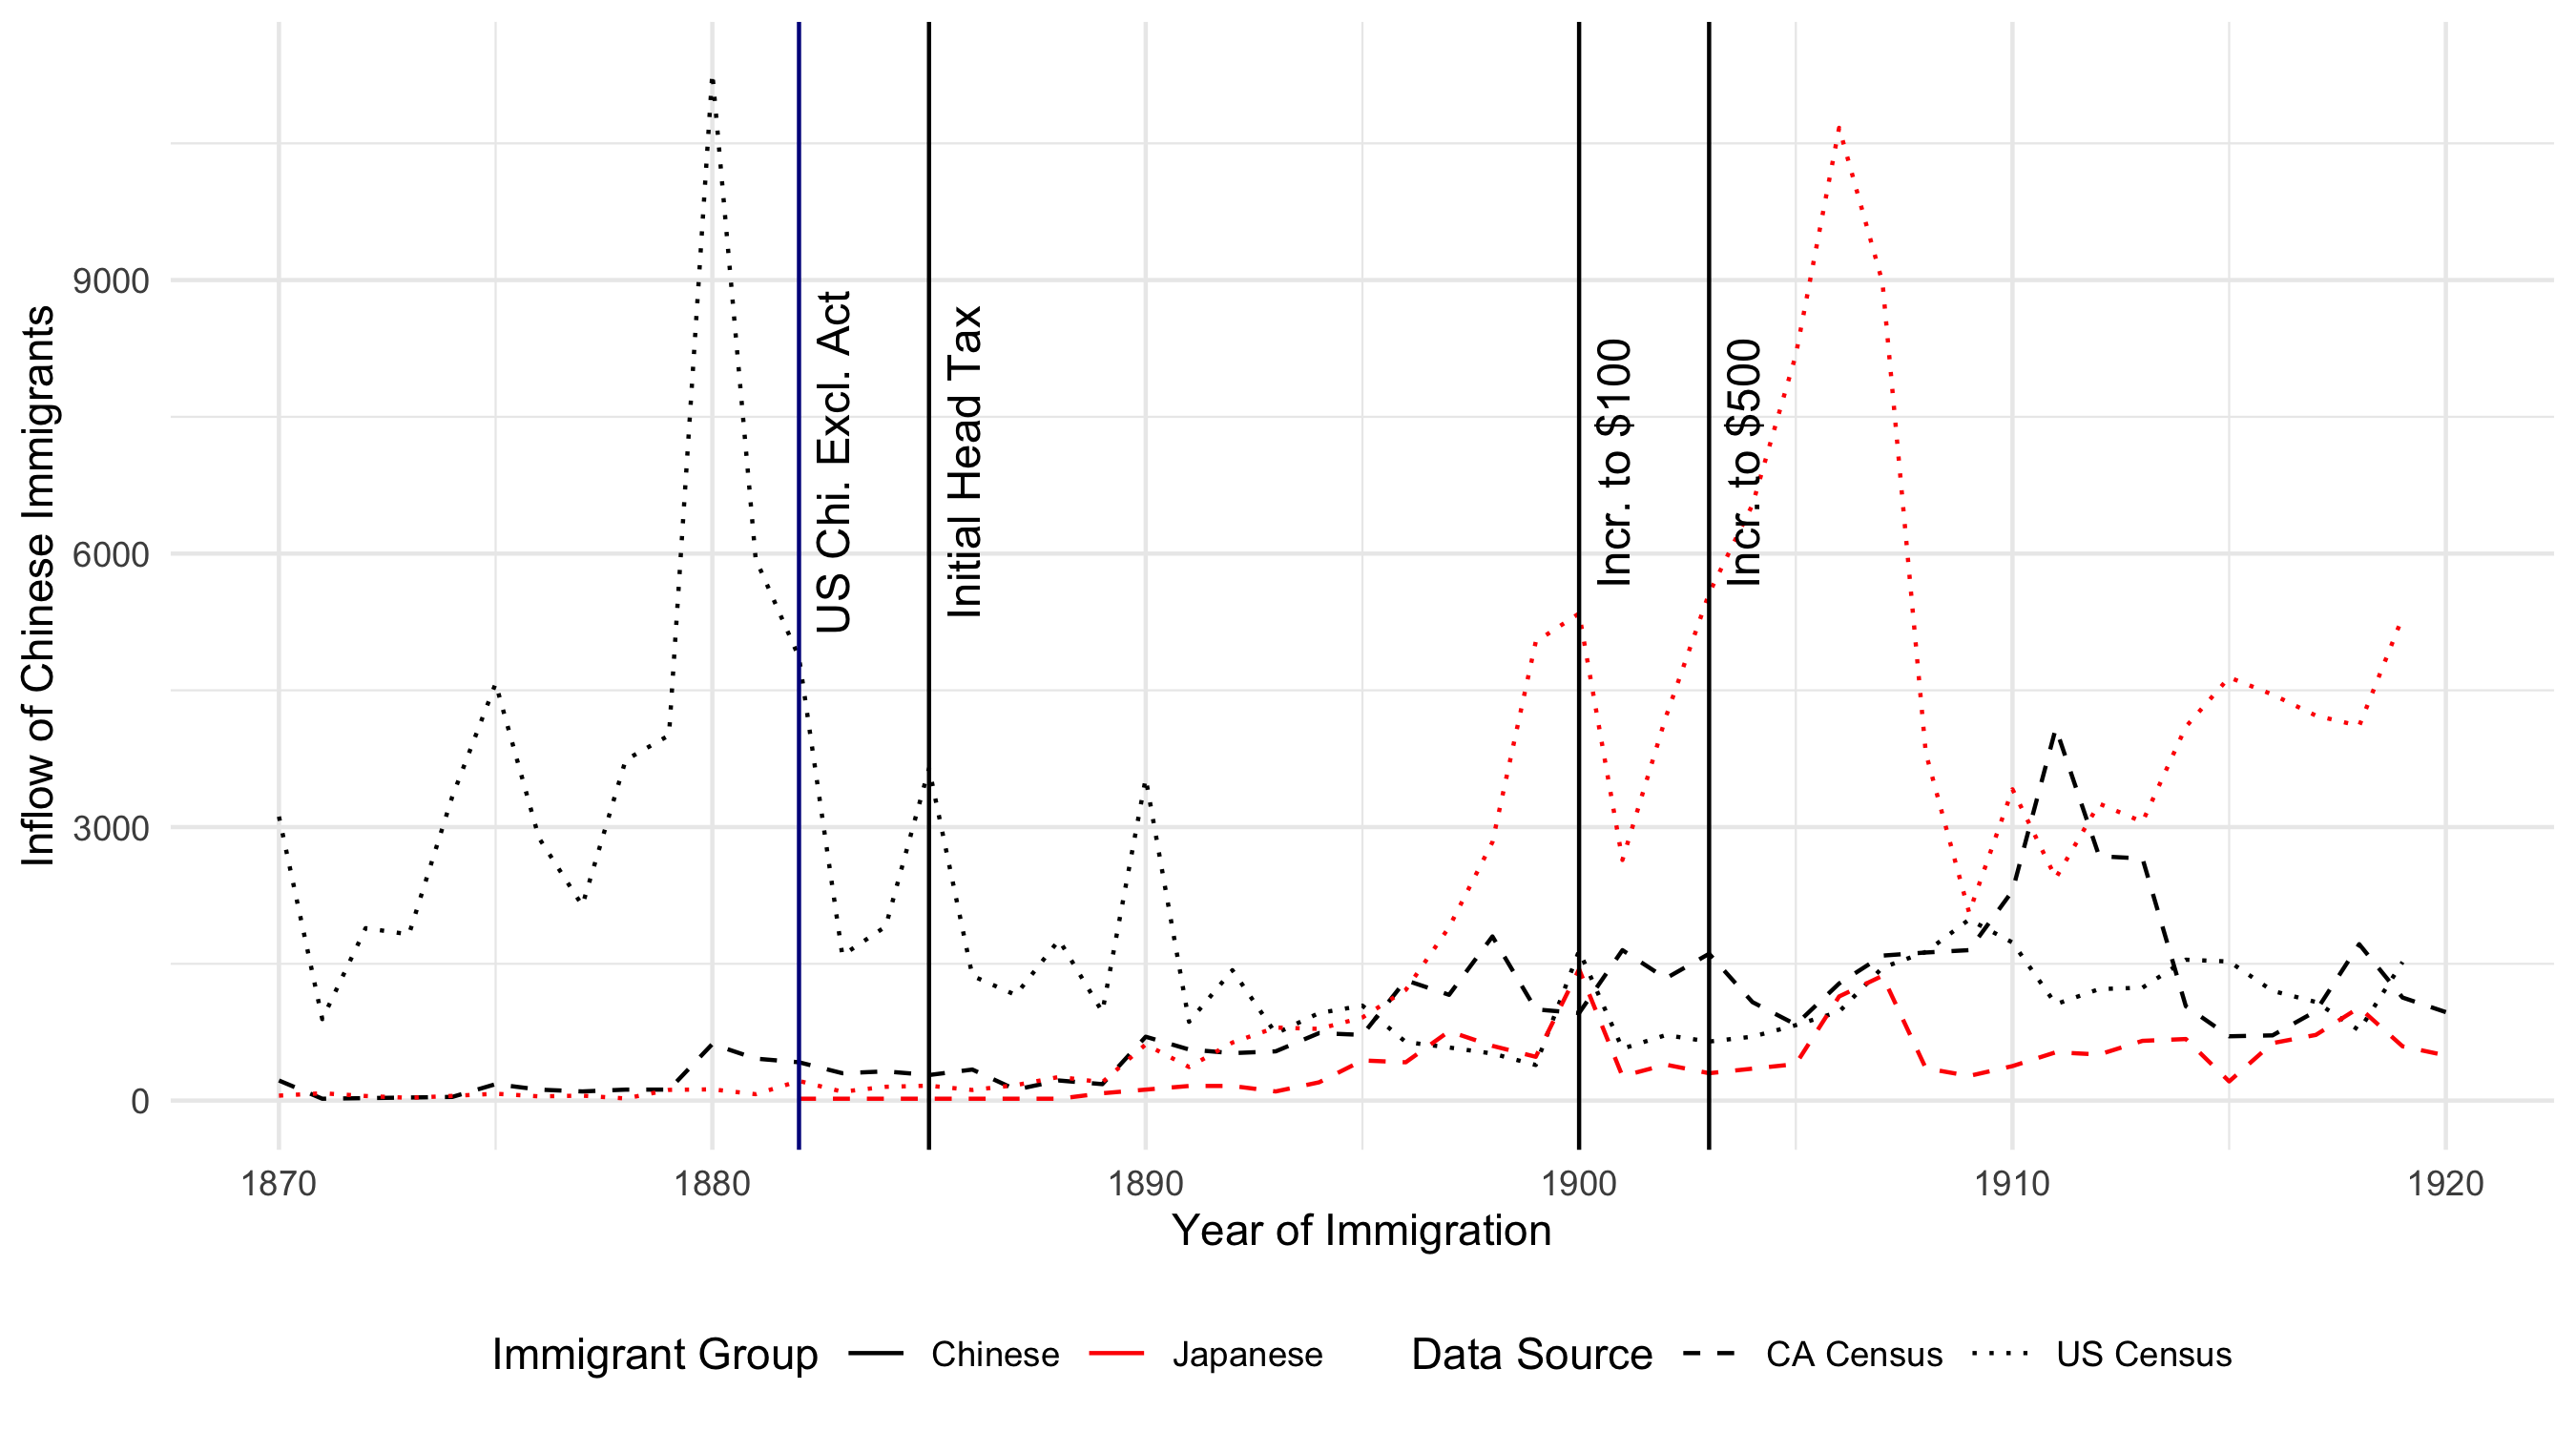
\includegraphics[width=\textwidth]{../../figs/fig3_us_can.png}
    \label{fig:taxpaid}
\end{figure}

The above analysis relies on the assumption above that in the absence of the head tax, the outcomes of Japanese and Chinese immigrants to Canada would have evolved similarly. In reality, it is likely that there were China-specific immigration shifters that would have affected Chinese immigration to Canada differently over time. In this section, I control for supply-side shocks by estimating the following equation:

\begin{multline}
    \label{eq:uscan}
    y_{ict} = \delta_{ct} + \sum_{c \in \{US, \, Canada\}} \alpha_c BORNCHI_i \times \mathbf{1}[COUNTRY_i = c] \\ + \sum_{k \in \{100,500\}, \, c \in \{US, \, Canada\}} \gamma_{ck} BORNCHI_i \times \mathbf{1}[COUNTRY_i = c] \times \mathbf{1}[TAX_t = k] + \varepsilon_{ict}
\end{multline}

where $c \in \{US, \, Canada\}$ indexes country, the coefficients $\alpha_c$ and $\gamma_{ck}$ now vary by country of arrival, and $\delta_{ct}$ now represents Year $\times$ Country fixed effects. 

\begin{table}[!h]
    \centering 
    \renewcommand{\arraystretch}{1.1}
    \resizebox{0.7\textwidth}{!}{
    \begin{threeparttable}
        \caption{Regression results from Equation \ref{eq:uscan} showing the relationship between the Chinese Head Tax and Chinese immigrant outcomes in Canada as compared to the US.}
        \label{tab:uscanregs}
        
% Table created by stargazer v.5.2.3 by Marek Hlavac, Social Policy Institute. E-mail: marek.hlavac at gmail.com
% Date and time: Sat, Apr 01, 2023 - 00:36:30
\begin{tabular}{@{\extracolsep{5pt}}lccc} 
\\[-1.8ex]\hline 
\hline \\[-1.8ex] 
 & \multicolumn{3}{c}{Sample: Chinese and Japanese Immigrants} \\ 
\cline{2-4} 
\\[-1.8ex] & LABORER & LITERATE & HOMEOWN \\ 
\\[-1.8ex] & (1) & (2) & (3)\\ 
\hline \\[-1.8ex] 
$BORNCHI \times US$ & $-$0.228$^{***}$ & $-$0.109$^{***}$ & $-$0.027$^{***}$ \\ 
& (0.009) & (0.007) & (0.006) \\ 
& & & \\ 
$BORNCHI \times CANADA $ & 0.252$^{***}$ & $-$0.057$^{***}$ & 0.041$^{***}$ \\ 
& (0.014) & (0.014) & (0.010) \\ 
& & & \\ 
$BORNCHI \times US \times $ \$100 Tax & 0.087$^{***}$ & 0.026$^{**}$ & $-$0.006 \\ 
& (0.014) & (0.012) & (0.010) \\ 
& & & \\ 
$BORNCHI \times US \times $ \$500 Tax & 0.062$^{***}$ & 0.048$^{***}$ & 0.012$^{*}$ \\ 
& (0.010) & (0.008) & (0.007) \\ 
& & & \\ 
$BORNCHI \times CANADA \times $ \$100 Tax & $-$0.256$^{***}$ & 0.298$^{***}$ & $-$0.114$^{***}$ \\ 
& (0.025) & (0.024) & (0.017) \\ 
& & & \\ 
$BORNCHI \times CANADA \times $ \$500 Tax & $-$0.112$^{***}$ & 0.010 & $-$0.118$^{***}$ \\ 
& (0.017) & (0.016) & (0.012) \\ 
& & & \\ 
Includes Year $\times$ Country FE & Yes & Yes & Yes \\ 
\hline \\[-1.8ex] 
Observations & 109,012 & 108,639 & 109,012 \\ 
Adjusted R$^{2}$ & 0.061 & 0.079 & 0.032 \\ 
\hline \\[-1.8ex] 
\end{tabular} 

        \begin{tablenotes}
            \item $^{*}$p$<$0.1; $^{**}$p$<$0.05; $^{***}$p$<$0.01
            \item 
            \item \textbf{Notes:} Analysis in this table uses Canadian census data from 1901-1921 and US census data from 1900-1920. As in Table \ref{tab:outcomes} I restrict the sample such that only immigrants who arrived after 1890 and prior to 1920 are included (since the latest US census year I use is 1920). All columns restrict the sample to only Chinese and Japanese immigrants from the US and Canada.
        \end{tablenotes}
    \end{threeparttable}
    }
\end{table}

Results of estimating Equation \ref{eq:uscan} for the sample of Chinese and Japanese immigrants to Canada who arrived between 1890 and 1920 are presented in Table \ref{tab:uscanregs}. Observe that Canadian Chinese immigrants are significantly less literate and more likely to be laborers than US Chinese immigrants, as suggested by summary statistics in Table \ref{tab:summstats}, and are also less likely to own their own home. Lines 3 and 4 represent the impact of Chinese immigrants to the US arriving in years with a higher \textbf{Canadian} head tax, which I would expect to be minimal, but I in fact observe to be significant. This suggests that the head tax may have had some spillover effects on Chinese immigration to the US. 

Column (1) shows that while Chinese immigrants to Canada in higher head tax years are less likely to be laborers (in line with the selection effect observed above), Chinese immigrants to the US in higher head tax years are in fact \textbf{more} likely to be laborers. This actually lends support to the selection theory, since the lower-skilled immigrants who could not afford the higher head tax may have substituted towards immigration to the US (although the existence of the Chinese Exclusion Act during this time period, which prohibited immigration of laborers, complicates this theory). 

Column (2) shows that immigrating in years with higher head taxes is associated with higher literacy rates for Chinese immigrants to both the US and Canada -- this is a puzzling result, as it does not accord with a theory of substitution between the US and Canada. Earnings are not included as an outcome variable because they are not available in the US census data during this time period, however column (3) presents results for home ownership. The results are again in line with my findings in Table \ref{tab:outcomes}, and the very small and mostly insignificant effects for Chinese immigrants to the US further suggests that the wealth effect (which does not affect Chinese immigrant outcomes in the US) dominates the selection effect (which would potentially spillover to Chinese immigrant outcomes in the US) for the outcome of home ownership.

\section{Conclusion}

In this paper, I find evidence that the Chinese Head Tax of 1885 had significant effects on the inflow of Chinese immigrants to Canada, as well as effects on selection into migration and wealth accumulation. While there is still a great deal of room to refine the analysis done in this paper, and to further investigate mechanisms, I believe that the initial findings give some initial insight into possible effects of the head tax, and the possible implications for present-day immigration policy. Selection into migration is a topic of great interest, and bears significant relevance to present-day immigration policies, many of which explicitly approve immigrants based on educational background and economic standing. Understanding how immigration costs, whether explicit (as in the case of the head tax), or implicit (as in the case of modern-day immigration), play a role in selection into migration and outcomes after arrival, is key to understanding how to best shape policy going forward. 


\newpage

\bibliography{../headtax.bib}


\end{document}
